\chapter{Mathematische Hilfsmittel}

\section{Skalar- und Vektorfelder}

Felder entsprechen Größen, die an jedem Raumpunkt einen bestimmten Wert haben, der zeitabhängig sein kann.\\ \linebreak

\begin{wrapfigure}[]{r}[0cm]{0cm}
	\raisebox{0pt}[\dimexpr\height-1\baselineskip\relax]{
		\colorbox{hgrey}{
			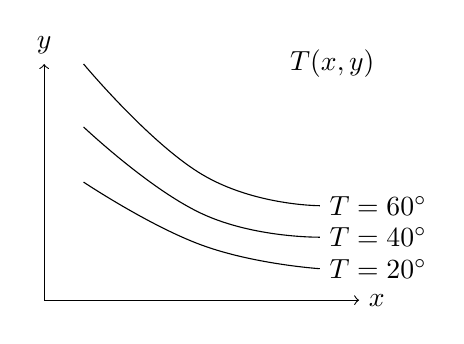
\begin{tikzpicture}
			\draw[->](0,0)-- (4,0) node[right]{$x$};
			\draw[->](0,0)--(0,3) node[above]{$y$};
			\draw (3,3) node[right]{$T(x,y)$};
			\draw plot[smooth, tension=.8] coordinates {(0.5,1.5)(2,0.7)(3.5,0.4)} node[right]{$T=20^{\circ}$} ;
			\draw plot[smooth, tension=.8] coordinates {(0.5,2.2)(2,1.1)(3.5,0.8)} node[right]{$T=40^{\circ}$} ;
			\draw plot[smooth, tension=.8] coordinates {(0.5,3)(2,1.6)(3.5,1.2)} node[right]{$T=60^{\circ}$} ;
			\end{tikzpicture}
		}
	}
	\caption{Isothermen}
\end{wrapfigure}

\textbf{a. skalare Felder}\ $\phi=\phi(x,y,z,t)$\\ 


Jedem Raumpunkt wird ein Wert in Form einer (reellen) Zahl zugeordnet, wie zum Beispiel Temperatur, Druck, Ladung oder Energie. Flächen oder Linien mit konstantem Wert nennt man Äquipotentialflächen beziehungsweise -linien.\\ \linebreak\linebreak

\begin{wrapfigure}[]{r}[0cm]{0cm}
	\raisebox{0pt}[\dimexpr\height-1\baselineskip\relax]{
		\colorbox{hgrey}{
			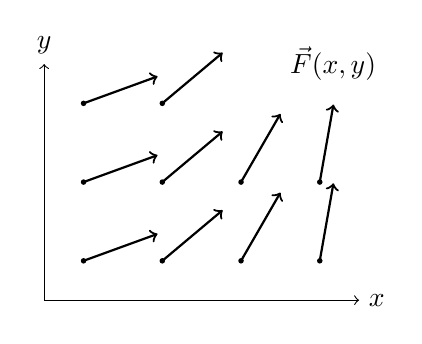
\begin{tikzpicture}
			
			\draw[->](0,0)-- (4,0) node[right]{$x$};
			\draw[->](0,0)--(0,3) node[above]{$y$};
			\draw (3,3) node[right]{$\vec{F}(x,y)$};
			\foreach \x/\angle in {0.5/20, 1.5/40} {
				\foreach \y in {0.5, 1.5, 2.5} {
					\fill (\x,\y) circle[radius=1pt];
					\draw[->,thick]  (\x, \y) -- ++(\angle:1);
				}
			}
			\foreach \x/\angle in {2.5/60, 3.5/80} {
				\foreach \y in {0.5, 1.5} {
					\fill (\x,\y) circle[radius=1pt];
					\draw[->,thick]  (\x, \y) -- ++(\angle:1);
				}
			}
			\end{tikzpicture}
		}
	}
	\caption{Kraftfeld}
\end{wrapfigure}


\textbf{b. Vektorfelder}\ $\vec{E}=\vec{E}(x,y,z,t)$\\

Jedem Raumpunkt wird ein Vektor zugeordnet, der lokal die Richtung des Feldes beschreibt, wie etwa ein Geschwindigkeits- oder Kraftfeld. Vektorfelder lassen sich durch Feldlinien veranschaulichen, entlang derer sich zum Beispiel ein Teilchen bewegt, das die entsprechende Kraft erfährt.


\section{Integrale auf Feldern}
Integrale über skalare Felder werden wie bekannt bebildet; sie sind zu vermeiden.\\
Integriert man über ein Vektorfeld, spielt die Richtungsinformation eine entscheidende Rolle. Man unterscheidet je nach Dimension des Parameterbereichs von Linien-, Flächen- und Volumenintegralen.\\
\linebreak


\textbf{a. Linienintegrale}

\begin{equation*}
\varphi=\int\limits_{C}\vec{E}(\vec{r})\d\vec{r}
\end{equation*}

\begin{wrapfigure}[]{r}[0cm]{0cm}
	\raisebox{0pt}[\dimexpr\height-1\baselineskip\relax]{
		\colorbox{hgrey}{
			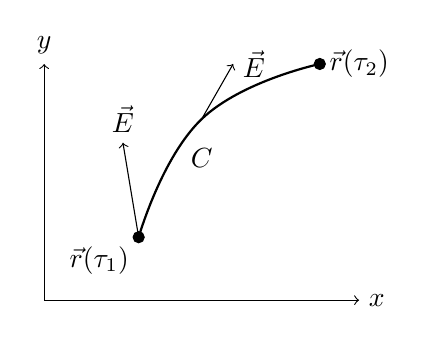
\begin{tikzpicture}
			
			\draw[->](0,0)-- (4,0) node[right]{$x$};
			\draw[->](0,0)--(0,3) node[above]{$y$};
			\draw[->](1.2,0.8)--(1,2) node[above]{$\vec{E}$};
			\draw[->](2,2.3)--(2.4,3) node[right]{$\vec{E}$};
			\draw(2,1.8) node{$C$};
			\draw[thick] plot[smooth, tension=.8] coordinates {(1.2,0.8)(2,2.3)(3.5,3)};
			\filldraw[black] (3.5,3) circle (2pt) node[right]{$\vec{r}(\tau_2)$};
			\filldraw[black] (1.2,0.8) circle (2pt) node[below left]{$\vec{r}(\tau_1)$};
			
			\end{tikzpicture}
		}
	}
	\caption{Linienintegral}
\end{wrapfigure}
Wir parametrisieren die Kurve durch $\vec{r}=\vec{r}(\tau)$ und erhalten somit
\begin{equation*}
\varphi=\int\limits_{\tau_0}^{\tau_1}\vec{E}(\vec{r}(\tau))\diff{\vec{r}}{\tau}\d \tau
\end{equation*}
Ein Speziallfall des Linienintegrals ist das sogenannte \textbf{geschlossene Linienintegral}, welches durch $\oint$ gekennzeichnet wird.\\
\linebreak


\begin{wrapfigure}[10]{r}[0cm]{0cm}
	\raisebox{0pt}[\dimexpr\height-1\baselineskip\relax]{
		\colorbox{hgrey}{
			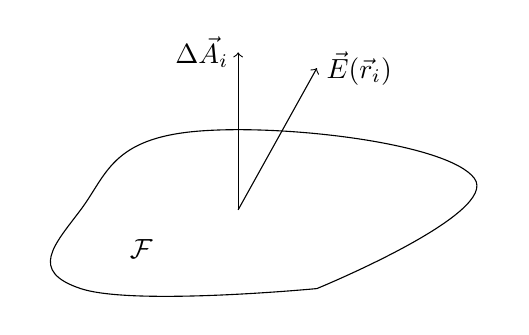
\begin{tikzpicture}
			
			\draw plot[smooth, tension=.8] coordinates {(3,0) (5,1.4) (1.5,2) (0,1) (0,0) (3,0) };	
			\draw[->] (2,1)--(2,3) node[left]{$\Delta\vec{A}_i$};
			\draw[->] (2,1)--(3,2.8) node[right]{$\vec{E}(\vec{r}_i)$};
			\draw (0.5,0.5) node[right]{$\mathcal{F}$};
			
			
			\end{tikzpicture}
		}
	}
	\caption{Flächenintegral}
\end{wrapfigure}


\textbf{b. Flächenintegrale}\\
\begin{equation*}
\Phi=\iint\limits_{S}\vec{B}\cdot\d \vec{A} \ \ \ \text{mit } \d\vec{A}=\d A\cdot\vec{n}
\end{equation*}


Ganz analog zu \textbf{a.} kann die Fläche $\vec{r}=\vec{r}(u,v)$ parametrisiert werden. Es ist jedoch beim Bilden der Funktionaldeterminante auf die Richtung des Flächenelements zu achten. Die beiden möglichen Lösungen unterscheiden sich natürlich nur um ein Vorzeichen. Wir erhalten also
\begin{equation*}
\Phi=\int\limits_{v_1}^{v_2}\int\limits_{u_1}^{u_2}\vec{B}(u,v)\cdot\left(\pdiff{\vec{r}}{u}\times\pdiff{\vec{r}}{v}\right)\d u\d v
\end{equation*}

\textbf{c. Volumenintegrale}\\
\linebreak
\begin{equation*}
Q=\iiint\limits_G\d V\cdot\rho(\vec{r})=\iiint\limits_G\d ^3 r\cdot\rho(\vec{r})=
\end{equation*}
Beim Volumenintegral wird wiederum (nicht wie beim Flächenintegral) das Vorzeichen des Volumenelements vernachlässigt, da physikalisch die \textbf{Richtung} des Volumens nur sehr selten wirklich von Bedeutung ist. Mit entsprechender Parametrisierung $\vec{r}=\vec{r}(u,v,w)$ ergibt sich
\begin{equation*}
q=\int\limits_{w_1}^{w_2}\int\limits_{v_1}^{v_2}\int\limits_{u_1}^{u_2}\rho(u,v,w)\cdot\left|\pdiff{\vec{r}}{u}\cdot\left(\pdiff{\vec{r}}{v}\times\pdiff{\vec{r}}{w}\right)\right|\d u\d v\d w
\end{equation*}

\section{Vektorielle Ableitungen und Integrale}
\textbf{a. Gradient}\\
\linebreak
Der Gradient $\grad\varphi\ $ eines Skalarfeldes beschreibt dessen Änderung und steht senkrecht auf den Äquipotentialflächen (oder allgemeiner: Niveaumengen). Der Gradient lässt sich durch den Nabla-Operator ausdrücken und lautet in karthesischen Koordinaten: 
\begin{equation*}
\nabla=\pdiff{}{x}\vec{e}_x+\pdiff{}{y}\vec{e}_y+\pdiff{}{z}\vec{e}_z
\end{equation*}
Wichtig ist, dass $\nabla$ ein vektorieller Differenzialoperator ist. Er folgt Ableitungsregeln, wie etwa der Kettenregel, und $\nabla\varphi$ verhält sich unter Koordinatentransformation wie ein Vektor.\\
\linebreak
Andere Schreibweisen: $\pdiff{}{\vec{r}},\ \partial_{\vec{r}},\ \nabla_{\vec{r}}$\\
\linebreak
\underline{Beispiele:}\\
\linebreak
$\nabla |\vec{r}|=\frac{\vec{r}}{|\vec{r}|}=\vec{e}_r\\
\nabla \frac{1}{|\vec{r}|}=-\frac{1}{r^2}\vec{e}_r$\\
\linebreak\linebreak
\textbf{b. Divergenz} (Quellenstärke eines Vektorfeldes)\\
\linebreak
Die Divergenz div $\vec{E}=\nabla\cdot\vec{E}$ ist ein Skalar unter Koordinatentransformation und kann als \textbf{lokale Quellenstärke} interpretiert werden. Häufig benötigt man auch den \textsc{Laplace}-Operator, der die \textbf{zweite Ableitung} repräsentiert.\\
\begin{equation*}
\div\grad \varphi \ = \ \nabla^2\varphi \ = \ \laplace\varphi
\end{equation*}
\underline{Beispiele:}\\
\linebreak
div $\vec{r}=3$ (Anzahl der Dimensionen)\\
div $(\varphi\vec{A})=\nabla\cdot(\varphi\vec{A})=\vec{A}(\nabla\varphi)+\varphi(\nabla\vec{A})=\vec{A}\cdot\grad \varphi+\varphi\cdot\div\vec{A}$\\
\linebreak
\textbf{c. Rotation} (Wirbelstärke eines Vektorfeldes)\\
\linebreak
Die Rotation rot $\vec{B}=\nabla\times\vec{B}$

\begin{equation*}
\nabla\times\vec{B}=\begin{vmatrix}
\vec{e}_x & \vec{e}_y & \vec{e}_z \\
\pdiff{}{x} & \pdiff{}{y} & \pdiff{}{z}\\
B_x & B_y & B_z
\end{vmatrix}
\end{equation*}

kann als \textbf{lokale Wirbelstärke} verstanden werden. Ihre Komponenten lassen sich auch als

\begin{equation*}
(\nabla\times\vec{B})_i=\sum\limits_{j,k}\epsilon_{ijk}\cdot\pdiff{}{x_j}\cdot B_k
\end{equation*}

darstellen wobei $\epsilon_{ijk}\ $ der total antisymetrische Tensor 3. Stufe ist.\\
\linebreak
\underline{Beispiele:}\\
\linebreak
$\vec{v}=\vec{\omega}\times\vec{r} \ \Rightarrow \ \nabla\times\vec{v}=2\vec{\omega}$\\
$\nabla\times\vec{r}=0$\\
\linebreak\linebreak
\textbf{d. \textsc{Gauss}'scher Satz}\\
\begin{equation*}
\iiint\limits_V\div\vec{E}\cdot\d V=\oiint\limits_{\partial V}\vec{E}\cdot\d \vec{A}
\end{equation*}
Der Satz von \textsc{Gauss} verknüpft Eigenschaften im Inneren eines Volumens mit dem Verhalten auf dem Rand.\\

Über den Satz von \textsc{Gauss} lässt sich auch die partielle Integration in drei Dimensionen umformen zu:

\begin{equation*}
\Int{V}{}{V} \ \pdiff{}{\vec{r}} (u\cdot v) = \Int{V}{}{V} \  \pdiff{u}{\vec{r}}\cdot v \ + \ \Int{V}{}{V} \  u \cdot\pdiff{v}{\vec{r}} \ = \ \Oiint{\partial V}{}{A} \  (u\cdot v)
\end{equation*}

\ \\
\textbf{e. \textsc{Green}'scher Satz}\\
\begin{equation*}
\Int{V}{}{(\varphi\laplace\psi-\psi\laplace\varphi)}{V}=\Oint{\partial V}{}{(\varphi\nabla\psi-\psi\nabla\varphi)}{\vec{A}}
\end{equation*}
\linebreak
\textbf{f. \textsc{Stokes}'scher Satz}\\
\begin{equation*}
\iint\limits_S\rot\vec{B}\cdot\d\vec{A}=\oint\limits_{\partial A}\vec{B}\cdot\d\vec{r}
\end{equation*}
Analog zu \textsc{Gauss}'schen Satz verknüft der Satz von \textsc{Stokes} das Verhalten eines Feldes auf einer Fläche mit dem auf dem Rand der Fläche. Für geschlossene Flächen gilt
\begin{equation*}
\oiint\limits_{S=\partial V}\rot\vec{B}\cdot\d\vec{A}=0
\end{equation*}

\section{Differentialoperatoren in krummlinigen Koordinaten}
Karthesische /Kugel-/Zylinderkoordinaten sind hier wichtig.\\
\linebreak
z.B: \ $\nabla_x\psi=\partial_x\psi\vec{e}_x+\partial_y\psi\vec{e}_y+\partial_z\psi\vec{e}_z$\\
\linebreak
$\nabla_\theta\psi=\pdiff{}{r}\psi\vec{e}_r+\frac{1}{r}\pdiff{}{\theta}\psi\vec{e}_\theta+\frac{1}{r\sin\theta}\pdiff{}{\phi}\psi\vec{e}_\phi$\\
\linebreak
Generell: $(\nabla\psi)_u\equiv(\nabla\psi)\vec{e}_u=\frac{1}{g_u}\pdiff{\psi}{u}$ \ mit \ $g_u=|\pdiff{\psi}{u}|$\\

\section{\textsc{Fourier}-Transformation}
\begin{equation*}
\tilde{f}(\omega)=\frac{1}{\sqrt{2\pi}}\Int{-\infty}{\infty}{f(t)e^{-i\omega t}}{t}
\end{equation*}
\begin{equation*}
f(t)=\frac{1}{\sqrt{2\pi}}\Int{-\infty}{\infty}{\tilde{f}(t)e^{i\omega t}}{\omega}
\end{equation*}
Verallgemeinert auf $n$ Dimensionen ergibt sich:\\
\begin{equation*}
\tilde{f}(\vec{k})=\frac{1}{({2\pi})^{\frac{n}{2}}}\Int{-\infty}{\infty}{f(\vec{r})e^{-i\vec{k}\vec{r}}}{^nr}
\end{equation*}
\linebreak
\textbf{a. Differentiation}\\
\begin{equation*}
\diff{}{t}f(t)=\frac{1}{\sqrt{2\pi}}\Int{-\infty}{\infty}{i\omega\tilde{f}(\omega)e^{i\omega t}}{\omega}
\end{equation*}
\linebreak
\textbf{b. Faltung}\\
\begin{equation*}
(f*g)(t)=\frac{1}{\sqrt{2\pi}}\Int{-\infty}{\infty}{f(t-s)G(s)}{s}
\end{equation*}
\begin{equation*}
\widetilde{(f*g)}(\omega)=\tilde{f}(\omega)\tilde{g}(\omega)
\end{equation*}
\textbf{c. Rechenregeln}\\
\begin{align*}
f'(t) & \leftrightarrow i\omega\tilde{f}(\omega)\\
-itf(t) & \leftrightarrow \tilde{f}'(\omega)\\
f(t+a) & \leftrightarrow  e^{i\omega a}\tilde{f}(\omega)\\
e^{i\omega t}f(t) &\leftrightarrow & \tilde{f}(\omega-a)\\
f(at) & \leftrightarrow \frac{1}{|a|}\tilde{f}\left(\frac{\omega}{a}\right)\\
f^*(t) & \leftrightarrow \tilde{f}^*(\omega)\\
\tilde{\tilde{f}}(t) &\leftrightarrow & f(-t)\\
\end{align*}

\section{Delta-Distribution}

Die Delta-Distribution ist über folgende Eigenschaften definiert:

\begin{enumerate}
	\item
	\begin{equation*}
	\delta(\vec{r}) = \begin{cases}
	0 & \text{für }\vec{r}\neq\vec{r}_0\\
	\infty & \text{für } \vec{r} = \vec{r}_0
	\end{cases}
	\end{equation*}
	
	\item
	\begin{equation*}
	\int\limits_{\vec{r}_0\in V}\d V \ \delta({\vec{r}-\vec{r}_0}) = 1
	\end{equation*}
\end{enumerate}

Alle Aussagen gelten analog für die Delta-Distribution $\delta(x)$ in einer Dimension.\
Bei höherdimensionalen Deltadistributionen gilt allerdings nur in kartesischen Koordinaten:

\begin{equation*}
\delta(\vec{r} - \vec{r}_0) = \delta(x-x_0)\cdot\delta(y-y_0)\cdot\delta(z-z_0)
\end{equation*}
\ \\
Faltet man die Delta-Distribution mit einer Funktion $f(\vec{r})$, so ergibt sich aus ihren Eigenschaften:

\begin{equation*}
\int\limits_{\vec{r}_0\in V}\d V \ \delta({\vec{r}-\vec{r}_0}) \ f(\vec{r}) = f(\vec{r}_0)
\end{equation*}

\section{\textsc{Green}'sche Funktion zur Lösung inhomogener linearer DGL}

Wir betrachten die lineare, inhomogene Differentialgleichung

\begin{equation*}
L \ \phi (x_1,\dotsc,x_n) = \rho (x_1,\dotsc,x_n) \; \text{ oder kurz } \; L\phi = \rho
\end{equation*}

wobei $L$ ein linearer Operator und $\rho$ die Inhomogenität sein soll.\
\\
Die \textsc{Green}'sche Funktion $G(x,x)$ zum Operator $L$ ist die Lösung der Differentialgleichung mit $\delta$-förmiger Inhomogenität.

\begin{equation*}
L \ G(x,x') = \delta (x-x') \; [= \delta(x_1-x_1')\cdot\dotsc\cdot\delta(x_n - x_n')]
\end{equation*}
\ \\
Wenn $g$ bekannt ist, dann kann die Lösung für beliebige Inhomogenität durch Superposition gewonnen werden.

\begin{equation*}
\phi (x) = \int\d x' \ G(x,x') \rho(x')
\end{equation*}

Den Beweis hierfür erhält man leicht durch Einsetzen:

\begin{equation*}
L \ \phi(x) = \int\d x' \ L \ G(x,x') \rho(x') = \rho(x)
\end{equation*}

